\subsection{Étude du contexte}

  \lettrine[nindent=0em,lines=3]{L}e but de ce projet sera dans un premier temps
  de mettre en place une infrastructure de compilation, de test et d'exécution
  d'un noyau Linux. La seconde partie du projet sera de comprendre comment
  fonctionne le noyau Linux au niveau de la mémoire, notamment pour la gestion
  des pages (emplacement, taille), et au niveau des processeurs pour le
  placement des threads et le parallélisme. Ensuite, il faudra se plonger dans
  la lecture du code et sa modification aux endroits adéquats en utilisant des
  technologies comme IBS où les hardware counters pour obtenir des informations
  précises sur la gestion des points évoqués ci-dessus. Enfin, pour tester ce
  noyau avec nos modifications, nous utiliserons la machine virtuelle et gdb
  pour le débugage.
  %% TODO: changer débugage par autre chose

  \subsubsection{Infrastructure}
    Dans cette partie, nous allons détailler l'infrastructure dont nous
    disposons et celle que nous avons mise en place pour ce projet. Notre avons
    à notre disposition une machine AMD Opteron 6172 composée de quatre
    processeurs à douze coeurs chacun cadencés à 2,1GHz et répartis en 8 noeuds
    avec 32G de mémoire vive. L'architecture des noeuds est la
    suivante\footnote{Source: \textit{Improving performance on NUMA systems},
      Baptiste Lepers}:

    %% TODO: vérifier l'archi à la main (méga chaud et méga long)

    %% node   0   1   2   3   4   5   6   7 
    %%   0:  10  16  16  22  16  22  16  22 
    %%   1:  16  10  16  22  22  16  22  16 
    %%   2:  16  16  10  16  16  16  16  22 
    %%   3:  22  22  16  10  16  16  22  16 
    %%   4:  16  22  16  16  10  16  16  16 
    %%   5:  22  16  16  16  16  10  22  22 
    %%   6:  16  22  16  22  16  22  10  16 
    %%   7:  22  16  22  16  16  22  16  10

    \begin{figure}[H]
      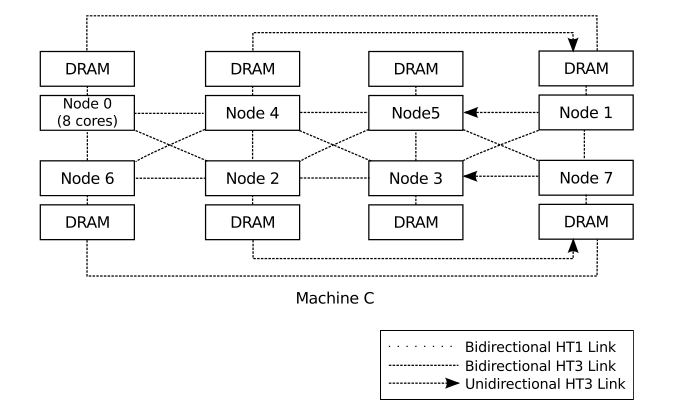
\includegraphics[scale=0.4]{img/numa_topology.png}
      \caption{Topologie de la machine 6172}
      \label{f:numa_topology}
    \end{figure}

    Sur cette machine, nous avons utilisé l'hyperviseur qemu, avec son extension
    kvm pour afin d'optimiser l'émulation. Afin d'améliorer encore plus cette
    dernière, nous avons utilisé le logiciel virt-manager qui détecte
    automatiquement la configuration matérielle de machine hôte et configure la
    machine virtuelle en conséquence. Cette configuration est à notre avis très
    réaliste puisqu'elle est capable d'activer/désactiver des options CPU comme
    la gestion d'IBS où l'hypervision. Un des autres avantage de virt-manager
    est que l'on peut sauvegarder la configuration dans un fichier, et pouvoir
    ainsi l'exporter facilement.

    Nous avons installé une machine virtuelle classique (Debian GNU/Linux), qui
    nous permettra par la suite de fournir à notre noyau compilé une
    architecture de base pour se lancer. En effet, la compilation du noyau se
    fera directement sur l'Opteron, mais le lancement et les tests se feront via
    l'hyperviseur. Afin que le noyau puisse se lancer et avoir une base, nous
    avons installé une première VM, donc nous récupérerons la configuration du
    noyau pour la compilation.

    Cette étape ne fût pas sans difficulté. Nous avons passé plus d'une semaine
    dessus, alors qu'il s'agit simplement d'installer une machine
    virtuelle. Malheureusement, l'université à eu des problèmes de réseux, et
    notamment de ssh la semaine six, le serveur a lui du être mis à jour, il y a
    eu des souçis de compatibilité de version de logiciels entre nos machines et
    le serveur, des souçis de virtualisation de matériel\ldots


  \subsubsection{Fonctionnement de la mémoire}
  
    TODO


  \subsubsection{Placement des threads}
    TODO

